\begin{figure}[t!]
	%=====================================================================%
	% yeo table
	%=====================================================================%
	\newcommand{\yeofont}[1]{\small{#1}}
	\setlength{\tabcolsep}{5.5pt}
	\renewcommand{\arraystretch}{0.97} % space between rows
	\captionof{table}{Network parcellation scheme of the brain proposed by Yeo \etal in \cite{Yeo:2011}.}
	\vspace{-6pt}\begin{tabular}{llll}
		\hline
		\multicolumn{4}{c}{\textbf{\small{Network membership Table ($\times$ is ``unlabeled'')}}}  \\ 
		\hline\hline
		 \yeofont{1. Visual}	& \yeofont{2. Somatomotor}	& \yeofont{3. Dorsal Attention} & \yeofont{4. Ventral Attention}  \\[-2pt]
		 \yeofont{5. Limbic} 	& \yeofont{\doblue{6. Frontoparietal}} & \yeofont{\dored{7. Default}} 	& \yeofont{8. Striatum} \\[-2pt]
		 \yeofont{9. Amygdala} & \yeofont{10. Hippocampus} & \yeofont{11. Thalamus}	& \yeofont{12. Cerebellum} \\[-1.5pt]
		\hline \\[-4pt]
	\end{tabular}
	%=====================================================================%
	% figures
	%=====================================================================%
	\renewcommand{\imwidth}{120pt}
	\renewcommand{\imheight}{61.0pt}
	\renewcommand{\arraystretch}{1.00} % space between rows
	\setlength{\tabcolsep}{3.85pt}	
	\renewcommand{\VSPACE}{\vspace{-100pt}}
	\begin{tabular}{cc}
		%=================================================================%
		% elastic net
		%=================================================================%
		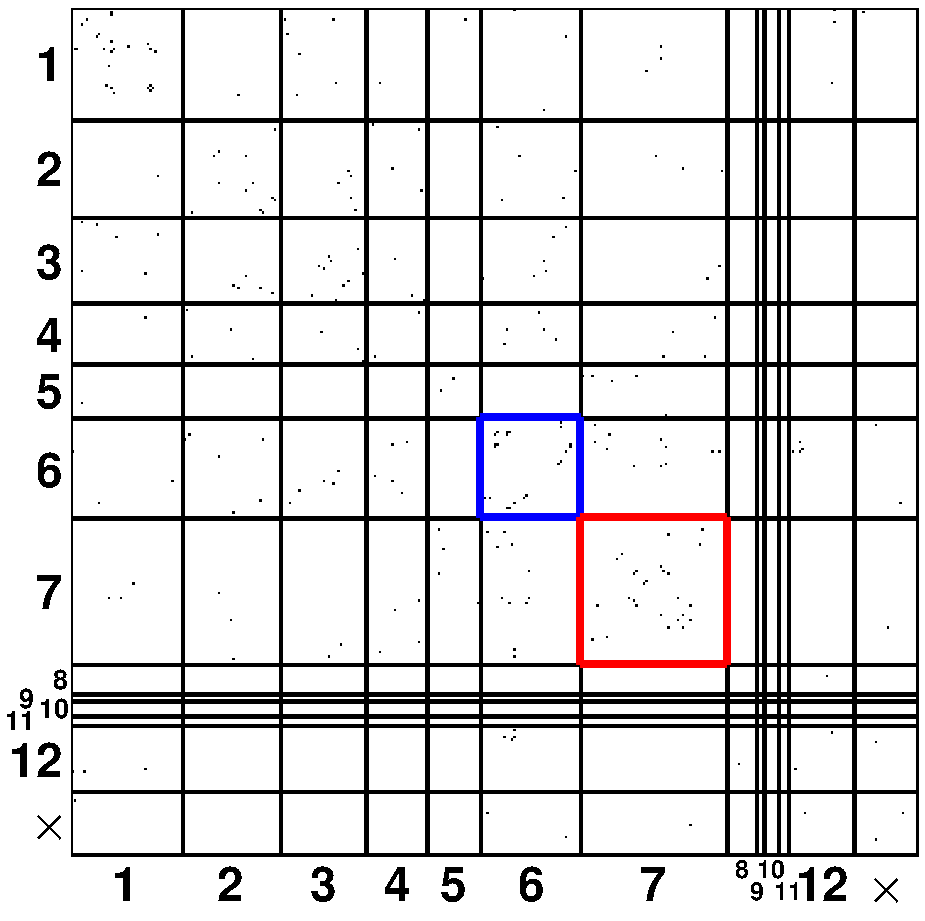
\includegraphics[width=\imwidth]{weight_enet.pdf} \hspace{1pt}
		&
		\begin{tabular}{ccc}
		\vspace{-135pt} \\
			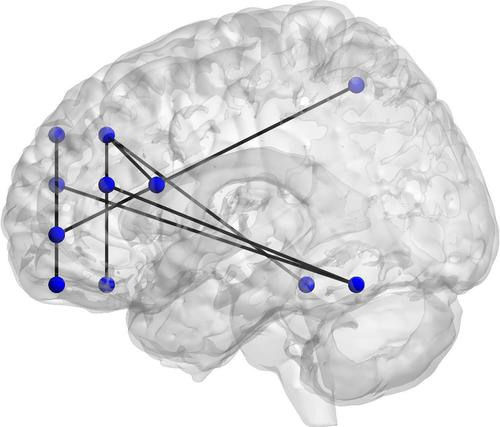
\includegraphics[height=\imheight]{6-6enet_lateral.jpg} & 
			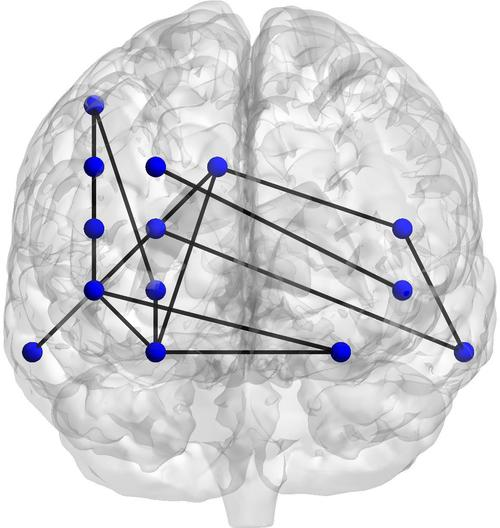
\includegraphics[height=\imheight]{6-6enet_anterior.jpg} & 
			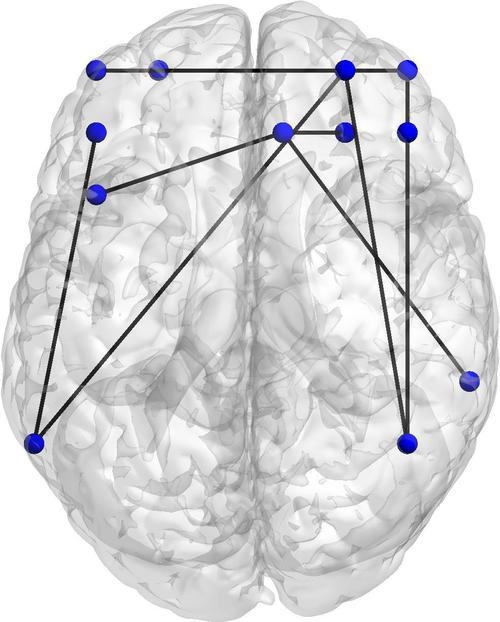
\includegraphics[height=\imheight]{6-6enet_superior.jpg} \\[-1.5pt]
			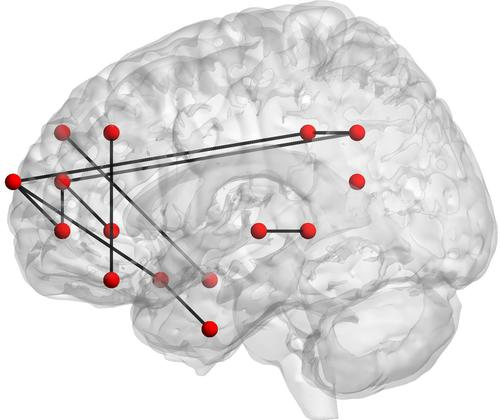
\includegraphics[height=\imheight]{7-7enet_lateral.jpg} & 
			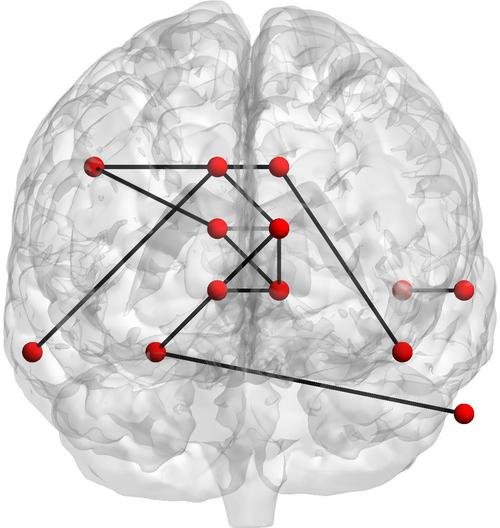
\includegraphics[height=\imheight]{7-7enet_anterior.jpg} & 
			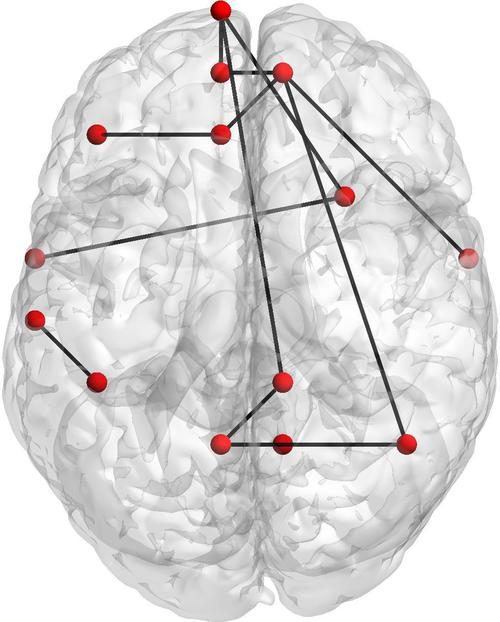
\includegraphics[height=\imheight]{7-7enet_superior.jpg} \\[-3.5pt]
		\end{tabular} \\[-0pt]
		\multicolumn{2}{c}{\small{\textbf{(a)} Multitask Elastic-net SVM result}}\\[12pt]
		%=================================================================%
		% fused lasso
		%=================================================================%
		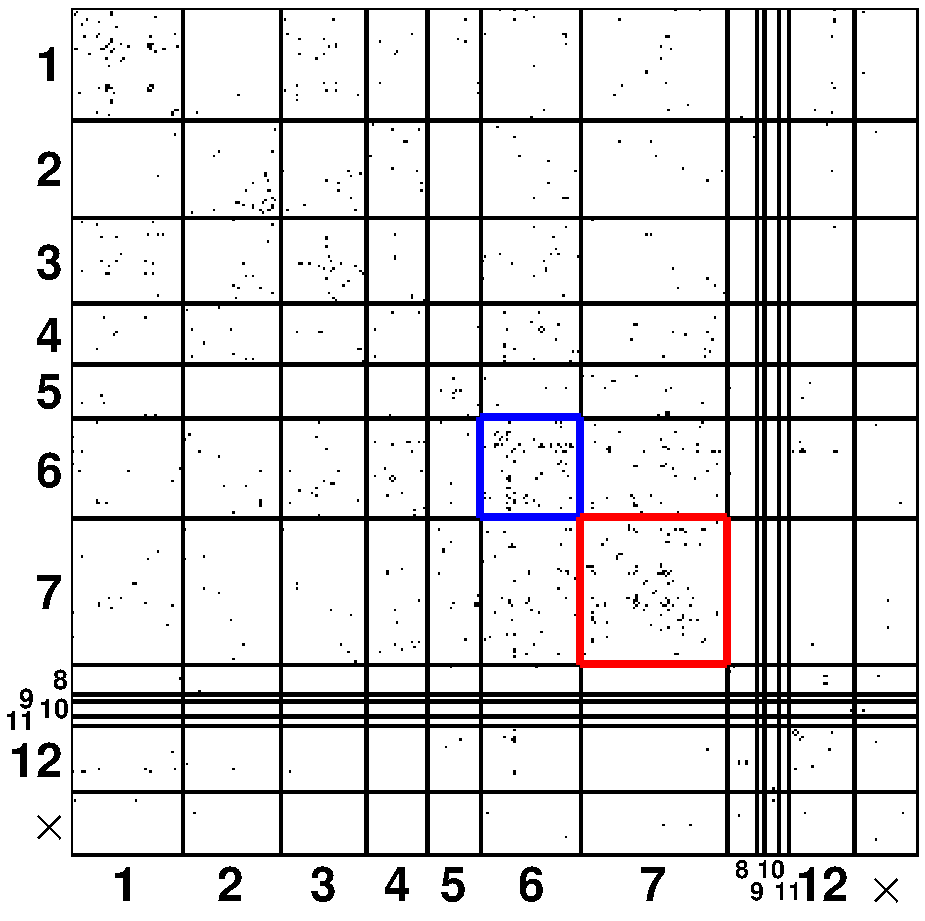
\includegraphics[width=\imwidth]{weight_flas.pdf} \hspace{1pt}
		&
		\begin{tabular}{ccc}
		\vspace{-135pt} \\
			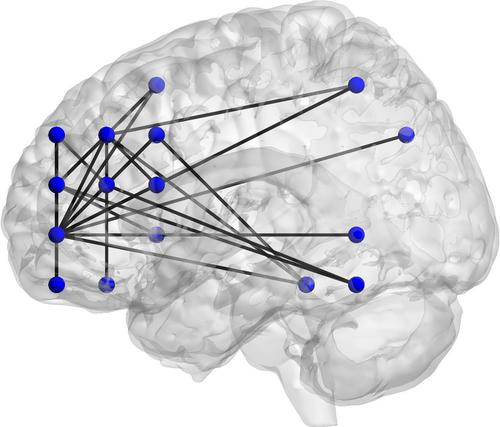
\includegraphics[height=\imheight]{6-6flas_lateral.jpg} & 
			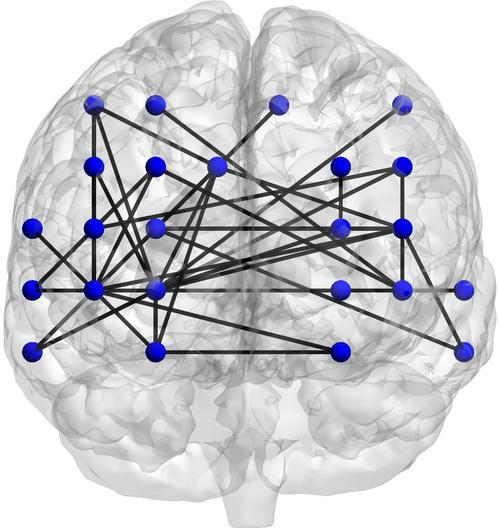
\includegraphics[height=\imheight]{6-6flas_anterior.jpg} & 
			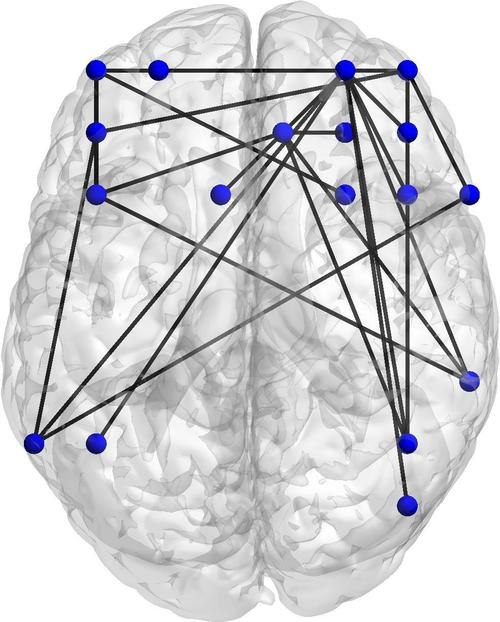
\includegraphics[height=\imheight]{6-6flas_superior.jpg} \\[-1.5pt]
			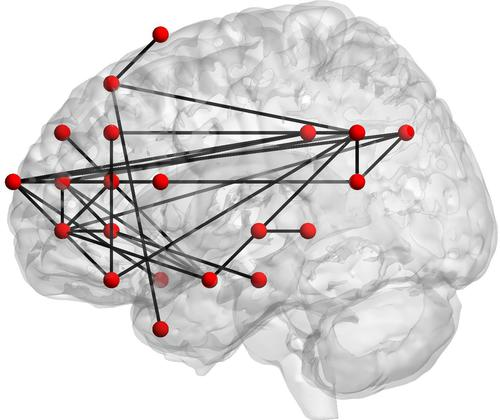
\includegraphics[height=\imheight]{7-7flas_lateral.jpg} & 
			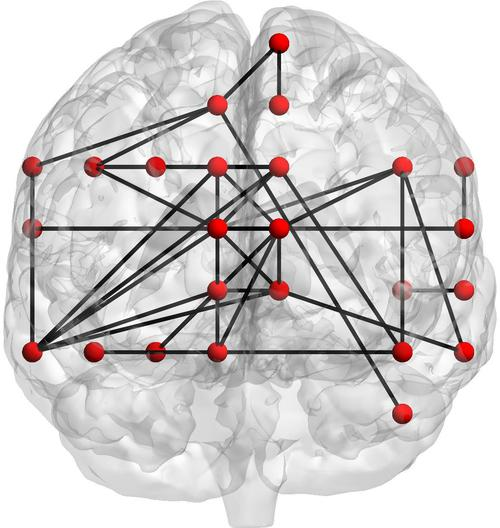
\includegraphics[height=\imheight]{7-7flas_anterior.jpg} & 
			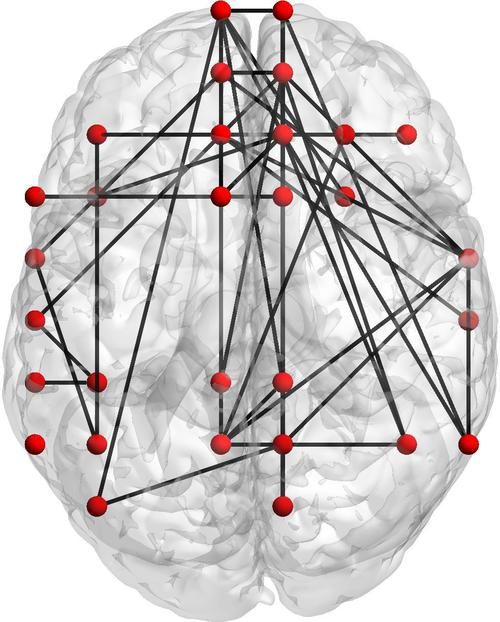
\includegraphics[height=\imheight]{7-7flas_superior.jpg} \\[-3.5pt]
		\end{tabular}  \\
		\multicolumn{2}{c}{\small{\textbf{(b)} Multitask Fused Lasso SVM result}}\\[3pt]
	\end{tabular} 
	\captionof{figure}{
	Weight vectors estimated from the EN+\MTL and FL+\MTL-penalized SVM.
	\textbf{Left:} support matrices of the selected features (rows/cols grouped by network membership).
	\textbf{Right:} brain space representation of the selected edges in the intra-frontoparietal (\mbox{6-6}: blue) and the intra-default network (7-7: red).
	}
	\label{fig:weight}
	\vspace{-14pt}
\end{figure}
